\section{Mean free path}
\label{sec:mean_free_path_calculation}
The mean free path $\lambda$ is the average distance a particle travels before it collides with another particle. We imagine a particle with diameter $d$ moving and find its \textit{effective collision area} to be (see figure \ref{fig:effective_collision_area})
\begin{align}
	A = \pi (2d)^2.
\end{align}
\begin{figure}[h]
\begin{center}
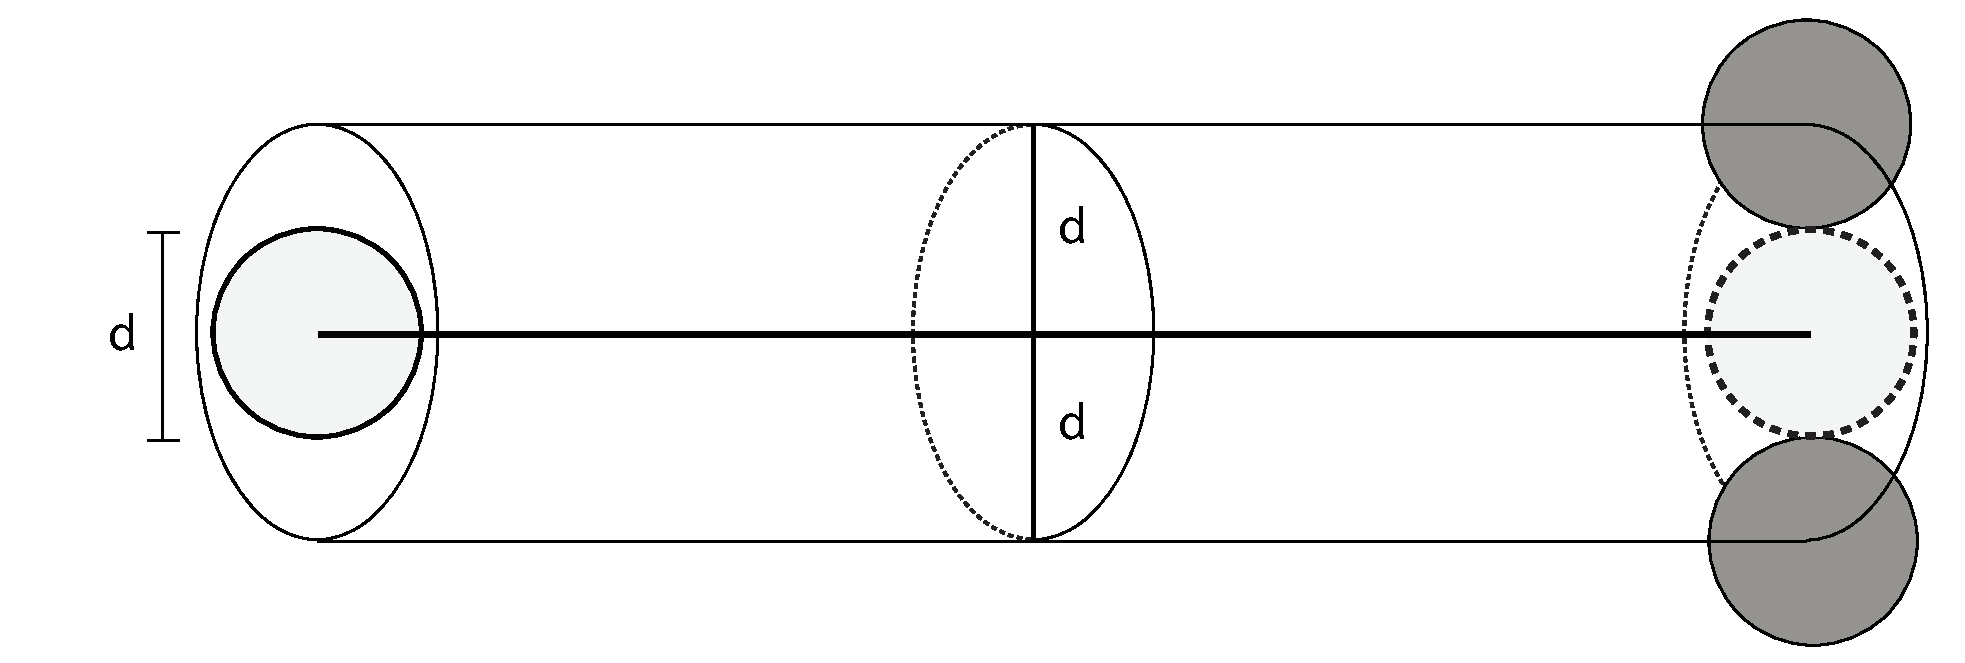
\includegraphics[width=0.8\textwidth, trim=0cm 0cm 0cm 0cm, clip]{DSMC/figures/effective_area2.eps}
\end{center}
\caption{A particle with diameter $d$ swipes out a cylinder with diameter $2d$, defining the collision area $A=\pi (2d)^2$ containing all points of which a collision partner can have its center in.}
\label{fig:effective_collision_area}
\end{figure}
Two particles $i$ and $j$, with velocities $\vec v_i$ and $\vec v_j$, have the relative velocity $\vec v_\text{rel} = \vec v_i - \vec v_j$. The norm is given as
\begin{align}
	v_\text{rel} &= \sqrt{\vec v_\text{rel}\cdot \vec v_\text{rel} } = \sqrt{ (\vec v_i - \vec v_j)(\vec v_i - \vec v_j)}\\
	&= \sqrt{\vec v_i\cdot \vec v_i - 2\vec v_i\vec v_j + \vec v_j\vec v_j},
\end{align}
from which we can find the average relative velocity by assuming that the velocities are completely random, and hence not correlated, and that the particles have the same mean speed $\langle v\rangle$
\begin{align}
	\langle v_\text{rel}\rangle &= \sqrt{\vec v_1^2 + \vec v_2^2} = \sqrt 2 \langle v\rangle,
\end{align}
During a time $\tau$, assuming average relative velocity $\sqrt 2 \langle v\rangle$, the total volume sweeped out by particle $i$ is 
\begin{align}
	V = \pi d^2\sqrt 2\langle v\rangle \tau,
\end{align}
which in turn gives the number of collisions during such a volume
\begin{align}
	\label{eq:num_collisions}
	n_\text{coll} = V\rho_n = \sqrt 2 \pi d^2\langle v\rangle \rho_n \tau,
\end{align}
where $\rho_n$ is the number density. The mean free path is then calculated as the length of the path divided by the number of collisions
\begin{align}
	\label{eq:mean_free_path}
	\lambda = \frac{\langle v\rangle \tau}{ \sqrt 2 \pi d^2\langle v\rangle \rho_n\tau} = \frac{1 }{ \sqrt 2 \pi d^2 \rho_n}.
\end{align}
\section{Mean collision time}
From the mean free path, it is easy to calculate the mean collision time. The mean collision time $\tau_\text{coll}$ is simply the average \textit{time} a particle travels before it collides with another particle. So, the mean free path was the distance $\lambda$ the average particle will travel. The average speed of the particles were $\langle v \rangle$, so $\tau_\text{coll}$ should then be
\begin{align}
	\label{eq:kinetic_theory_mean_collision_time}
	\tau_\text{coll} &= \frac{\lambda}{\langle v\rangle} = \frac{1}{\sqrt 2 \pi d^2 \rho_n \langle v \rangle}\\
	&= \sqrt{\frac{m\pi}{k_B T}}\frac{1}{4\pi d^2\rho_n},
\end{align}
where we have used the expression for the average velocity (equation \eqref{eq:maxwell_boltzmann_average_speed}). 